\documentclass[11pt]{article}

\usepackage[letterpaper,margin=1in,top=1in,bottom=1in]{geometry}
\usepackage{amsmath,amssymb}
\usepackage{tikz}
\usepackage{enumitem}
\usepackage{fancyhdr}
\usepackage{lastpage}
\usepackage[most]{tcolorbox}
\usepackage{array}
\usepackage{titlesec}
\usepackage{xcolor}

% ---- Colors ----
\definecolor{fangblue}{RGB}{20,60,110}
\definecolor{fanggray}{RGB}{90,90,90}
\definecolor{boxgray}{RGB}{245,245,245}

% ---- Header / Footer ----
\pagestyle{fancy}
\fancyhf{}
\renewcommand{\headrulewidth}{0.4pt}
\renewcommand{\footrulewidth}{0.4pt}
\lhead{\small\itshape Graphing Quadratics: Domain \& Range}
\rhead{\small\itshape FangMath}
\lfoot{\small\textcopyright\ 2026 FangMath $\cdot$ All rights reserved.}
\rfoot{\small\thepage}

% ---- Section headings ----
\titleformat{\section}{\large\bfseries\color{fangblue}}{\thesection.}{0.6em}{}
\titleformat{\subsection}{\normalsize\bfseries}{}{0em}{}
\setlength{\parindent}{0pt}
\setlength{\parskip}{4pt}

% ---- Key formula box ----
\newtcolorbox{keybox}{colback=boxgray,colframe=fangblue,boxrule=0.6pt,
  arc=2pt,left=8pt,right=8pt,top=6pt,bottom=6pt}

% ---- X-method helper: #1 product (top), #2 left, #3 right, #4 sum (bottom) ----
\newcommand{\xmethod}[4]{%
\begin{tikzpicture}[scale=0.62,baseline=(current bounding box.center)]
  \draw[thick] (-0.9,0.9)--(0.9,-0.9);
  \draw[thick] (0.9,0.9)--(-0.9,-0.9);
  \node at (0,1.25) {\footnotesize #1};
  \node[left]  at (-1.0,0) {\footnotesize #2};
  \node[right] at (1.0,0)  {\footnotesize #3};
  \node at (0,-1.25) {\footnotesize #4};
\end{tikzpicture}}

% ---- Graph grid helper ----
\newcommand{\blankgrid}[1]{%
\begin{tikzpicture}[scale=0.5]
  \draw[step=1,gray!30,very thin] (-5,-5) grid (5,5);
  \draw[->,thick] (-5,0)--(5,0) node[right]{\scriptsize $x$};
  \draw[->,thick] (0,-5)--(0,5) node[above]{\scriptsize $y$};
  \foreach \n in {-4,-2,2,4}{\draw (\n,0.12)--(\n,-0.12) node[below]{\tiny \n};}
  \foreach \n in {-4,-2,2,4}{\draw (0.12,\n)--(-0.12,\n) node[left]{\tiny \n};}
  #1
\end{tikzpicture}}

\begin{document}

% ================= TITLE BLOCK =================
\begin{center}
  {\LARGE\bfseries\color{fangblue} Graphing Quadratic Functions:\\[2pt] Domain \& Range}\\[6pt]
  {\color{fanggray} Notes $\cdot$ Summary $\cdot$ Practice Problems $\cdot$ Full Answer Key}
\end{center}

\vspace{4pt}
\begin{center}
\begin{tabular}{@{}p{7.5cm}@{\hspace{1cm}}p{5cm}@{}}
\textbf{Name:} \underline{\hspace{5cm}} & \textbf{Date:} \underline{\hspace{3.5cm}}
\end{tabular}
\end{center}
\begin{center}\small\itshape Estimated time: 40--55 minutes\end{center}

\vspace{6pt}
\hrule
\vspace{10pt}

% ================= 1. SUMMARY =================
\section{Summary}

A \textbf{quadratic function} has the form $y = ax^2 + k$ (with $a \neq 0$). Its graph is a
\textbf{parabola} --- a U-shaped curve.

\textbf{Direction.} If $a > 0$ the parabola opens \emph{up}; if $a < 0$ it opens \emph{down}.
The larger $|a|$ is, the \emph{narrower} the parabola; the smaller $|a|$ is, the \emph{wider} it is.

\textbf{Vertex.} For $y = ax^2 + k$ the vertex (turning point) is at $(0,\,k)$. This is the lowest
point when the parabola opens up, and the highest point when it opens down.

\textbf{Domain} = the set of all allowed $x$-values (inputs). \\
\textbf{Range} = the set of all resulting $y$-values (outputs).

\begin{keybox}
\textbf{Key facts for $y = ax^2 + k$:}
\begin{itemize}[nosep,leftmargin=1.4em]
\item \textbf{Domain: all real numbers}, $(-\infty,\infty)$ --- you may square any number.
\item If $a>0$: \textbf{Range} is $y \ge k$, i.e. $[k,\infty)$.
\item If $a<0$: \textbf{Range} is $y \le k$, i.e. $(-\infty,k]$.
\end{itemize}
\end{keybox}

\textbf{How do we find the domain?} Use a number line and ask: can $x$ be zero? negative?
positive? For a plain parabola the answer is \emph{yes} to all three, so the domain is all
real numbers.

\vspace{4pt}
\begin{center}
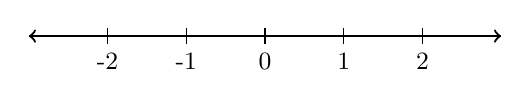
\begin{tikzpicture}[scale=1]
  \draw[<->,thick] (-3,0)--(3,0);
  \foreach \n in {-2,-1,0,1,2}{\draw (\n,0.1)--(\n,-0.1) node[below]{\small \n};}
\end{tikzpicture}
\end{center}

% ================= 2. WORKED EXAMPLES =================
\section{Worked Examples}

\subsection{Example --- graph $y = \dfrac{1}{3}x^2$}

Build a table of values. Remember $x^2$ means $x \cdot x$, so a negative input gives a positive
output:
\[
y = \tfrac{1}{3}(-3)^2 = \tfrac{1}{3}\,(-3)(-3) = \tfrac{1}{3}(9) = 3.
\]

\begin{center}
\begin{minipage}{4cm}
\centering
\renewcommand{\arraystretch}{1.2}
\begin{tabular}{c|c}
$x$ & $y$ \\ \hline
$-3$ & $3$ \\
$0$  & $0$ \\
$3$  & $3$
\end{tabular}
\end{minipage}
\hspace{0.6cm}
\begin{minipage}{7cm}
\centering
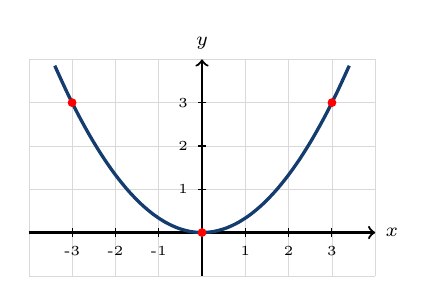
\begin{tikzpicture}[scale=0.55]
  \draw[step=1,gray!30,very thin] (-4,-1) grid (4,4);
  \draw[->,thick] (-4,0)--(4,0) node[right]{\scriptsize $x$};
  \draw[->,thick] (0,-1)--(0,4) node[above]{\scriptsize $y$};
  \foreach \n in {-3,-2,-1,1,2,3}{\draw (\n,0.1)--(\n,-0.1) node[below]{\tiny \n};}
  \foreach \n in {1,2,3}{\draw (0.1,\n)--(-0.1,\n) node[left]{\tiny \n};}
  \draw[domain=-3.4:3.4,smooth,variable=\x,fangblue,very thick] plot ({\x},{\x*\x/3});
  \filldraw[red] (-3,3) circle (2.5pt) (0,0) circle (2.5pt) (3,3) circle (2.5pt);
\end{tikzpicture}
\end{minipage}
\end{center}

Since $a=\tfrac13>0$ the parabola opens up with vertex $(0,0)$.
\[
\boxed{\text{Domain: all real numbers } (-\infty,\infty)} \qquad
\boxed{\text{Range: } y \ge 0,\ [0,\infty)}
\]

\subsection{Example --- a downward, shifted parabola $y = -x^2 + 2$}

Here $a=-1<0$, so it opens down; the vertex is $(0,2)$, the \emph{highest} point.
\[
\boxed{\text{Domain: all real numbers}} \qquad
\boxed{\text{Range: } y \le 2,\ (-\infty,2]}
\]

\subsection{Example --- comparing the width of parabolas}

Compare $f(x) = -x^2$, \quad $g(x) = 3x^2$, \quad $h(x) = -\dfrac{1}{3}x^2$.

Line up the coefficients and take their \textbf{absolute values} --- the sign only tells you
which way the parabola opens, not how wide it is:
\[
\text{coefficients: } -1,\ \ 3,\ \ -\tfrac13
\qquad\Longrightarrow\qquad
|a|:\ \ 1,\ \ 3,\ \ \tfrac13 .
\]

\begin{keybox}
\textbf{Width rule.} When comparing the width of parabolas, use only $|a|$ (the absolute value
of the coefficient):
\begin{itemize}[nosep,leftmargin=1.4em]
\item The \textbf{greater} $|a|$ is, the \textbf{narrower} the parabola.
\item The \textbf{smaller} $|a|$ is, the \textbf{wider} the parabola.
\end{itemize}
\end{keybox}

So from narrowest to widest: $g$ ($|a|=3$), then $f$ ($|a|=1$), then $h$ $\big(|a|=\tfrac13\big)$.

\textit{Still confused?} Graph $y=\dfrac{1}{7}x^2$ next to $y=x^2$ on the same axes. The small
coefficient $\tfrac17$ makes a much wider, flatter parabola --- confirming: smaller $|a|$
$\Rightarrow$ wider.

\begin{center}
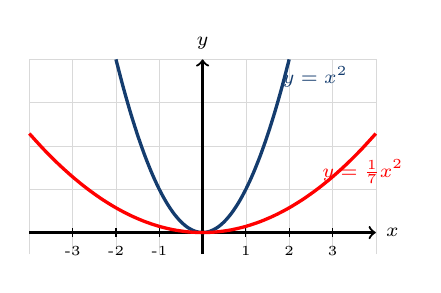
\begin{tikzpicture}[scale=0.55]
  \draw[step=1,gray!30,very thin] (-4,-0.5) grid (4,4);
  \draw[->,thick] (-4,0)--(4,0) node[right]{\scriptsize $x$};
  \draw[->,thick] (0,-0.5)--(0,4) node[above]{\scriptsize $y$};
  \foreach \n in {-3,-2,-1,1,2,3}{\draw (\n,0.1)--(\n,-0.1) node[below]{\tiny \n};}
  \draw[domain=-2:2,smooth,variable=\x,fangblue,very thick] plot ({\x},{\x*\x});
  \node[fangblue] at (2.6,3.6) {\scriptsize $y=x^2$};
  \draw[domain=-4:4,smooth,variable=\x,red,very thick] plot ({\x},{\x*\x/7});
  \node[red] at (3.7,1.4) {\scriptsize $y=\frac17x^2$};
\end{tikzpicture}
\end{center}

\begin{keybox}
\textbf{Conclusion.} The width of a parabola $y=ax^2$ depends only on $|a|$, not on its sign.
A \textbf{greater} $|a|$ gives a \textbf{narrower} graph; a \textbf{smaller} $|a|$
gives a \textbf{wider} graph. The sign of $a$ only decides whether the parabola opens up or down.
\end{keybox}

\subsection{Example --- vertical shifts $y = ax^2 + c$}

\textbf{How is the graph of $y = 3x^2 + 2$ different from the graph of $y = 3x^2$?}

Make a table and compare the two columns --- every $y$-value is exactly $2$ larger:

\begin{center}
\renewcommand{\arraystretch}{1.2}
\begin{tabular}{c|c|c}
$x$ & $y = 3x^2$ & $y = 3x^2 + 2$ \\ \hline
$-2$ & $12$ & $14$ \\
$-1$ & $3$  & $5$  \\
$0$  & $0$  & $2$  \\
$1$  & $3$  & $5$  \\
$2$  & $12$ & $14$
\end{tabular}
\end{center}

The parabola $y = 3x^2 + 2$ has the \emph{same shape} as $y = 3x^2$, but every point is lifted
straight up $2$ units. \textbf{It is shifted 2 units up.}

\begin{keybox}
\textbf{Vertical-shift rule.} Adding $c$ to $y = ax^2$ slides the whole parabola up or down
without changing its shape:
\begin{itemize}[nosep,leftmargin=1.4em]
\item If $c > 0$: shift \textbf{up} $c$ units; the vertex moves to $(0,c)$.
\item If $c < 0$: shift \textbf{down} $|c|$ units; the vertex moves to $(0,c)$.
\end{itemize}
\end{keybox}

\subsection{Example --- solving $x^2 = k$ by square roots}

To solve $x^2 = 16$, take the square root of \emph{both sides}. The key is that
$\sqrt{x^2} = |x|$ (not just $x$), because squaring erases a negative sign:
\[
x^2 = 16 \;\Longrightarrow\; \sqrt{x^2} = \sqrt{16} \;\Longrightarrow\; |x| = 4
\;\Longrightarrow\; x = \pm 4 \quad(\text{i.e. } x = 4 \text{ or } x = -4).
\]

That is why a square-root equation has \textbf{two} solutions: both $4$ and $-4$ square to $16$.

\begin{keybox}
\textbf{Square-root rule.} If $x^2 = k$ with $k > 0$, then $x = \pm\sqrt{k}$ (two solutions).
If $k = 0$, then $x = 0$ (one solution). If $k < 0$, there is \textbf{no real solution},
since a square is never negative.
\end{keybox}

\subsection{Example --- solving by graphing}

To solve an equation like $x^2 + c = 0$, graph the \textbf{related function} $y = x^2 + c$ and
read off its \textbf{$x$-intercepts} (where $y = 0$). Each $x$-intercept is a solution.

\begin{center}
% A: y = x^2 - 4  (two solutions)
\begin{minipage}{0.31\textwidth}\centering
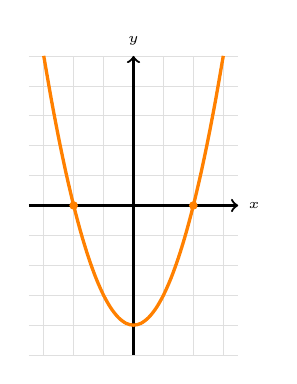
\begin{tikzpicture}[scale=0.38]
  \draw[step=1,gray!25,very thin] (-3.5,-5) grid (3.5,5);
  \draw[->,thick] (-3.5,0)--(3.5,0) node[right]{\tiny $x$};
  \draw[->,thick] (0,-5)--(0,5) node[above]{\tiny $y$};
  \draw[domain=-3:3,smooth,variable=\x,orange,very thick] plot ({\x},{\x*\x-4});
  \filldraw[orange] (-2,0) circle (3.5pt) (2,0) circle (3.5pt);
\end{tikzpicture}\\[2pt]
{\footnotesize \textbf{A.} $x^2-4=0$\\ $y=x^2-4$\\ Two solutions: $x=\pm 2$}
\end{minipage}\hfill
% B: y = x^2  (one solution)
\begin{minipage}{0.31\textwidth}\centering
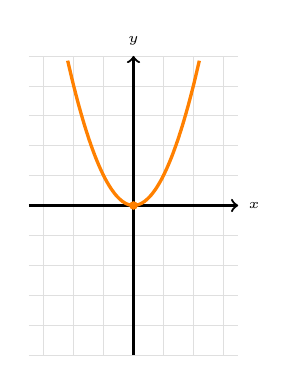
\begin{tikzpicture}[scale=0.38]
  \draw[step=1,gray!25,very thin] (-3.5,-5) grid (3.5,5);
  \draw[->,thick] (-3.5,0)--(3.5,0) node[right]{\tiny $x$};
  \draw[->,thick] (0,-5)--(0,5) node[above]{\tiny $y$};
  \draw[domain=-2.2:2.2,smooth,variable=\x,orange,very thick] plot ({\x},{\x*\x});
  \filldraw[orange] (0,0) circle (3.5pt);
\end{tikzpicture}\\[2pt]
{\footnotesize \textbf{B.} $x^2=0$\\ $y=x^2$\\ One solution: $x=0$}
\end{minipage}\hfill
% C: y = x^2 + 2  (no solution)
\begin{minipage}{0.31\textwidth}\centering
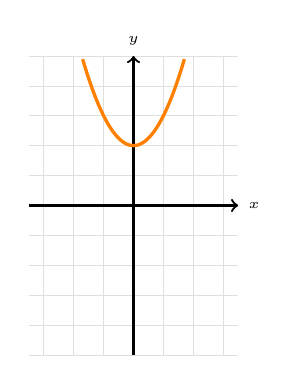
\begin{tikzpicture}[scale=0.38]
  \draw[step=1,gray!25,very thin] (-3.5,-5) grid (3.5,5);
  \draw[->,thick] (-3.5,0)--(3.5,0) node[right]{\tiny $x$};
  \draw[->,thick] (0,-5)--(0,5) node[above]{\tiny $y$};
  \draw[domain=-1.7:1.7,smooth,variable=\x,orange,very thick] plot ({\x},{\x*\x+2});
\end{tikzpicture}\\[2pt]
{\footnotesize \textbf{C.} $x^2+2=0$\\ $y=x^2+2$\\ No real solution}
\end{minipage}
\end{center}

\begin{keybox}
\textbf{Solving by graphing.} The real solutions of $ax^2 + c = 0$ are the $x$-intercepts of
the related graph $y = ax^2 + c$. A parabola can cross the $x$-axis \textbf{twice} (two solutions),
\textbf{touch} it once (one solution), or \textbf{miss} it entirely (no real solution).
\end{keybox}

\subsection{Example --- factoring $ax^2 + bx + c$ (product--sum method)}

Factor $2a^2 - 15a + 18$. When the leading coefficient is not $1$, use the \textbf{``X''} method:

\begin{enumerate}[leftmargin=1.6em,itemsep=2pt]
\item Multiply the outer terms: $2a^2 \cdot 18 = 36a^2$ (top of the X). For simplicity we
      drop the $a^2$ and just use $\mathbf{36}$.
\item The middle term is $-15a$; for simplicity we use $-15$ as the sum (bottom of the X).
      Find two numbers whose \textbf{product} is $36$ and whose \textbf{sum} is $-15$.
      They are $-3$ and $-12$.
\item Split the middle term using those numbers and factor by grouping:
\end{enumerate}
\[
2a^2 - 15a + 18 = 2a^2 - 3a - 12a + 18 = a(2a - 3) - 6(2a - 3) = (2a - 3)(a - 6).
\]

\begin{center}
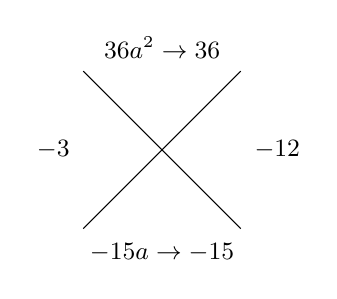
\begin{tikzpicture}[scale=1]
  \draw (-1,1)--(1,-1); \draw (1,1)--(-1,-1);
  \node at (0,1.3) {\small $36a^2 \to 36$};
  \node at (0,-1.3) {\small $-15a \to -15$};
  \node[left] at (-1.05,0) {\small $-3$};
  \node[right] at (1.05,0) {\small $-12$};
\end{tikzpicture}
\end{center}

\textbf{Check:} $(2a-3)(a-6) = 2a^2 - 12a - 3a + 18 = 2a^2 - 15a + 18$. \checkmark

\begin{keybox}
\textbf{Product--sum rule.} To factor $ax^2 + bx + c$: find two numbers that multiply to
$a\cdot c$ and add to $b$. Use them to split the middle term, then factor by grouping.
\end{keybox}

\newpage
% ================= 3. PRACTICE =================
\section{Practice Problems}

For each function: make a table of at least three points, sketch the parabola on the grid,
and state the \textbf{domain} and \textbf{range}.

% ---------- EASY ----------
\subsection*{Part A --- Easy \hfill \normalfont\itshape (basic $y = ax^2$)}

\textit{Model.}\ \ $y = 3x^2$: points $(-1,3),(0,0),(1,3)$; opens up, vertex $(0,0)$.
Domain: all reals $(-\infty,\infty)$; Range: $y \ge 0$, $[0,\infty)$.

\vspace{6pt}
\begin{minipage}[t]{0.48\textwidth}
\textbf{A1.}\quad $y = x^2$\\[2pt]
Domain: \underline{\hspace{3.2cm}}\\[2pt]
Range: \underline{\hspace{3.5cm}}
\end{minipage}\hfill
\begin{minipage}[t]{0.48\textwidth}
\centering\blankgrid{}
\end{minipage}

\vspace{10pt}
\begin{minipage}[t]{0.48\textwidth}
\textbf{A2.}\quad $y = 2x^2$\\[2pt]
Domain: \underline{\hspace{3.2cm}}\\[2pt]
Range: \underline{\hspace{3.5cm}}
\end{minipage}\hfill
\begin{minipage}[t]{0.48\textwidth}
\centering\blankgrid{}
\end{minipage}

\vspace{10pt}
\begin{minipage}[t]{0.48\textwidth}
\textbf{A3.}\quad $y = \dfrac{1}{2}x^2$\\[6pt]
Domain: \underline{\hspace{3.2cm}}\\[2pt]
Range: \underline{\hspace{3.5cm}}
\end{minipage}\hfill
\begin{minipage}[t]{0.48\textwidth}
\centering\blankgrid{}
\end{minipage}

\vspace{10pt}
\begin{minipage}[t]{0.48\textwidth}
\textbf{A4.}\quad $y = -x^2$\\[2pt]
Domain: \underline{\hspace{3.2cm}}\\[2pt]
Range: \underline{\hspace{3.5cm}}
\end{minipage}\hfill
\begin{minipage}[t]{0.48\textwidth}
\centering\blankgrid{}
\end{minipage}

\newpage
% ---------- MEDIUM ----------
\subsection*{Part B --- Medium \hfill \normalfont\itshape (vertical shifts and reflections $y = ax^2 + k$)}

\textit{Model.}\ \ $y = 2x^2 - 3$: opens up (since $a>0$), vertex $(0,-3)$.
Domain: all reals; Range: $y \ge -3$, $[-3,\infty)$.

\vspace{6pt}
\begin{minipage}[t]{0.48\textwidth}
\textbf{B1.}\quad $y = x^2 + 2$\\[2pt]
Vertex: \underline{\hspace{2.2cm}}\\[2pt]
Domain: \underline{\hspace{3.2cm}}\\[2pt]
Range: \underline{\hspace{3.5cm}}
\end{minipage}\hfill
\begin{minipage}[t]{0.48\textwidth}
\centering\blankgrid{}
\end{minipage}

\vspace{10pt}
\begin{minipage}[t]{0.48\textwidth}
\textbf{B2.}\quad $y = -2x^2$\\[2pt]
Vertex: \underline{\hspace{2.2cm}}\\[2pt]
Domain: \underline{\hspace{3.2cm}}\\[2pt]
Range: \underline{\hspace{3.5cm}}
\end{minipage}\hfill
\begin{minipage}[t]{0.48\textwidth}
\centering\blankgrid{}
\end{minipage}

\vspace{10pt}
\begin{minipage}[t]{0.48\textwidth}
\textbf{B3.}\quad $y = \dfrac{1}{3}x^2 - 1$\\[6pt]
Vertex: \underline{\hspace{2.2cm}}\\[2pt]
Domain: \underline{\hspace{3.2cm}}\\[2pt]
Range: \underline{\hspace{3.5cm}}
\end{minipage}\hfill
\begin{minipage}[t]{0.48\textwidth}
\centering\blankgrid{}
\end{minipage}

\vspace{10pt}
\begin{minipage}[t]{0.48\textwidth}
\textbf{B4.}\quad $y = -x^2 + 4$\\[2pt]
Vertex: \underline{\hspace{2.2cm}}\\[2pt]
Domain: \underline{\hspace{3.2cm}}\\[2pt]
Range: \underline{\hspace{3.5cm}}
\end{minipage}\hfill
\begin{minipage}[t]{0.48\textwidth}
\centering\blankgrid{}
\end{minipage}

\newpage
% ---------- HARD ----------
\subsection*{Part C --- Hard \hfill \normalfont\itshape (reasoning \& applications)}

\textit{Model.}\ \ State the domain and range of $y = 3x^2 - 2$ without graphing:
$a=3>0$ so it opens up; the constant $-2$ is the vertex $y$-value (a minimum).
Domain: all reals; Range: $y \ge -2$, $[-2,\infty)$.

\vspace{6pt}
\textbf{C1.} Without graphing, state the domain and range of $y = -\dfrac{1}{2}x^2 + 3$.
Explain how you knew the range from the equation alone.
\vspace{2.2cm}

\textbf{C2.} A parabola opens \emph{upward} and its lowest point is $(0,-5)$. Write a possible
equation, then give its domain and range.
\vspace{2.2cm}

\textbf{C3.} Two students disagree. One says the range of $y = x^2$ is ``all real numbers'' because
the domain is all real numbers. Explain why that is wrong and give the correct range.
\vspace{2.2cm}

\textbf{C4.} \textbf{Application.} A ball is thrown and its height (in feet) after $t$ seconds is
$h = -16t^2 + 4$. Physically, what values of $t$ make sense (the domain), and what is the
greatest height the ball reaches (top of the range)?
\vspace{2.5cm}

\subsection*{Part D --- Comparing Width (uses $|a|$)}

\textit{Model.}\ \ Order $y=4x^2$, $y=x^2$, $y=\tfrac13 x^2$ from narrowest to widest:
$|a|=4,\,1,\,\tfrac13$, so narrowest $\to$ widest is $4x^2$, then $x^2$, then $\tfrac13 x^2$.

\vspace{6pt}
\textbf{D1.} \emph{(Easy)}\ \ Order these from \textbf{widest to narrowest} using only $|a|$:
\[
f(x) = 5x^2, \qquad g(x) = x^2, \qquad h(x) = \tfrac{1}{4}x^2.
\]
\vspace{1.4cm}

\textbf{D2.} \emph{(Medium)}\ \ For $f(x) = -x^2$, \ $g(x) = 3x^2$, \ $h(x) = -\tfrac{1}{3}x^2$,
write each $|a|$ and order the graphs from narrowest to widest. Does the negative sign change
the width? Explain.
\vspace{1.8cm}

\textbf{D3.} \emph{(Hard)}\ \ A parabola is \emph{wider} than $y = x^2$ but \emph{narrower} than
$y = \tfrac{1}{10}x^2$, and it opens \emph{down}. Write one possible equation and state its $|a|$.
\vspace{2cm}

\subsection*{Part E --- Vertical Shifts $y = ax^2 + c$}

For each, describe how the graph differs from the base parabola (shift direction and number
of units), and give the new vertex.

\textit{Model.}\ \ How is $y = 4x^2 - 1$ different from $y = 4x^2$? It is shifted \textbf{down 1}
unit (same shape); new vertex $(0,-1)$.

\vspace{6pt}
\textbf{E1.}\ \ How is $y = 3x^2 + 4$ different from $y = 3x^2$?
\vspace{1.3cm}

\textbf{E2.}\ \ How is $y = x^2 - 5$ different from $y = x^2$?
\vspace{1.3cm}

\textbf{E3.}\ \ How is $y = -2x^2 + 1$ different from $y = -2x^2$?
\vspace{1.3cm}

\textbf{E4.}\ \ How is $y = \tfrac{1}{2}x^2 - 3$ different from $y = \tfrac{1}{2}x^2$?
\vspace{1.3cm}

\textbf{E5.}\ \ Graph $y = x^2$ and $y = x^2 + 2$ on the same axes. How are the two graphs related?
\vspace{1.6cm}

\subsection*{Part F --- Solving $x^2 = k$ by Square Roots}

Solve each equation. Give all real solutions (remember $x = \pm\sqrt{k}$).

\textit{Model.}\ \ $x^2 = 64 \Rightarrow |x| = 8 \Rightarrow x = \pm 8$.

\vspace{6pt}
\textit{Easy.}\quad
\textbf{F1.}\ \ $x^2 = 9$ \hspace{3cm} \textbf{F2.}\ \ $x^2 = 49$
\vspace{1.4cm}

\textit{Medium.}\quad
\textbf{F3.}\ \ $3x^2 = 48$ \hspace{2.4cm} \textbf{F4.}\ \ $x^2 = 20$
\vspace{1.4cm}

\textit{Hard.}\quad
\textbf{F5.}\ \ $(x-1)^2 = 9$ \hspace{2.2cm} \textbf{F6.}\ \ $x^2 = -16$
\vspace{1.6cm}

\subsection*{Part G --- Solving by Graphing}

For each equation, graph the related function and state the solutions (how many, and what
they are).

\textit{Model.}\ \ $x^2 - 1 = 0$: the related graph $y = x^2 - 1$ crosses the $x$-axis at $-1$
and $1$, so there are \textbf{two solutions}, $x = \pm 1$.

\vspace{6pt}
\textbf{G1.}\ \ $x^2 - 9 = 0$
\vspace{1.4cm}

\textbf{G2.}\ \ $2x^2 + 8 = 0$
\vspace{1.4cm}

\textbf{G3.}\ \ $x^2 - 49 = -49$
\vspace{1.6cm}

\subsection*{Part H --- Factoring $ax^2 + bx + c$ (product--sum method)}

Factor each trinomial completely. Check by multiplying back.

\textit{Model.}\ \ Factor $2x^2 + 5x + 2$. The product of the outer terms is
$2x^2 \cdot 2 = 4x^2$; for simplicity we drop the $x^2$ and use $4$. The middle term is $5x$;
likewise we use $5$ for the sum. Find two numbers with product $4$ and sum $5$: $1$ and $4$.
\quad\raisebox{-1.1em}{\xmethod{$4x^2 \to 4$}{$1$}{$4$}{$5x \to 5$}}
\[
2x^2 + 5x + 2 = 2x^2 + x + 4x + 2 = x(2x+1) + 2(2x+1) = (2x+1)(x+2).
\]

\vspace{6pt}
\textit{Easy.}\quad
\textbf{H1.}\ \ $2x^2 + 7x + 3$ \hspace{2.4cm} \textbf{H2.}\ \ $3x^2 + 8x + 4$
\vspace{1.6cm}

\textit{Medium.}\quad
\textbf{H3.}\ \ $3x^2 - 10x + 8$ \hspace{2.2cm} \textbf{H4.}\ \ $5x^2 + 13x + 6$
\vspace{1.6cm}

\textit{Hard.}\quad
\textbf{H5.}\ \ $6x^2 - 7x - 3$ \hspace{2.4cm} \textbf{H6.}\ \ $4x^2 - 4x - 15$
\vspace{1.8cm}

\newpage
% ================= 4. ANSWER KEY =================
\section{Detailed Answer Key}

\subsection*{Part A --- Easy}
\begin{description}[leftmargin=2.4em,style=nextline,itemsep=3pt]
\item[A1.] $y=x^2$: opens up, vertex $(0,0)$.\quad Domain: all reals $(-\infty,\infty)$;\ Range: $y\ge 0$, $[0,\infty)$.
\item[A2.] $y=2x^2$: narrower, opens up, vertex $(0,0)$.\quad Domain: all reals;\ Range: $y\ge 0$, $[0,\infty)$.
\item[A3.] $y=\tfrac12 x^2$: wider, opens up, vertex $(0,0)$.\quad Domain: all reals;\ Range: $y\ge 0$, $[0,\infty)$.
\item[A4.] $y=-x^2$: opens down, vertex $(0,0)$.\quad Domain: all reals;\ Range: $y\le 0$, $(-\infty,0]$.
\end{description}

\subsection*{Part B --- Medium}
\begin{description}[leftmargin=2.4em,style=nextline,itemsep=3pt]
\item[B1.] $y=x^2+2$: opens up, vertex $(0,2)$.\quad Domain: all reals;\ Range: $y\ge 2$, $[2,\infty)$.
\item[B2.] $y=-2x^2$: opens down (narrow), vertex $(0,0)$.\quad Domain: all reals;\ Range: $y\le 0$, $(-\infty,0]$.
\item[B3.] $y=\tfrac13 x^2-1$: opens up (wide), vertex $(0,-1)$.\quad Domain: all reals;\ Range: $y\ge -1$, $[-1,\infty)$.
\item[B4.] $y=-x^2+4$: opens down, vertex $(0,4)$.\quad Domain: all reals;\ Range: $y\le 4$, $(-\infty,4]$.
\end{description}

\subsection*{Part C --- Hard}
\begin{description}[leftmargin=2.4em,style=nextline,itemsep=5pt]
\item[C1.] $a=-\tfrac12<0$ so the parabola opens down; the constant $+3$ is the vertex $y$-value, which is the maximum. \textbf{Domain:} all reals $(-\infty,\infty)$; \textbf{Range:} $y\le 3$, $(-\infty,3]$.
\item[C2.] Opens up with minimum $(0,-5)$, so $k=-5$ and any $a>0$ works, e.g. $y=x^2-5$. \textbf{Domain:} all reals; \textbf{Range:} $y\ge -5$, $[-5,\infty)$.
\item[C3.] Domain and range are different questions. Squaring any real number gives a result $\ge 0$, so $y$ can never be negative. The correct \textbf{range} is $y\ge 0$, $[0,\infty)$ --- not all reals.
\item[C4.] Time starts at release and ends when the ball lands ($h=0$): $-16t^2+4=0 \Rightarrow t^2=\tfrac14 \Rightarrow t=\tfrac12$. Physical \textbf{domain:} $0\le t\le \tfrac12$ seconds. The parabola opens down with vertex at $t=0$, so the greatest height is $h=4$ feet.
\end{description}

\subsection*{Part D --- Comparing Width}
\begin{description}[leftmargin=2.4em,style=nextline,itemsep=5pt]
\item[D1.] $|a|$ values are $5,\ 1,\ \tfrac14$. Widest $\to$ narrowest (smallest $|a|$ first): $h(x)=\tfrac14x^2$, then $g(x)=x^2$, then $f(x)=5x^2$.
\item[D2.] $|a|$ values: $f\!:1,\ g\!:3,\ h\!:\tfrac13$. Narrowest $\to$ widest: $g$ ($3$), $f$ ($1$), $h$ ($\tfrac13$). The negative sign does \emph{not} change width --- it only flips the parabola to open downward. Width depends only on $|a|$.
\item[D3.] Need $\tfrac{1}{10} < |a| < 1$ and $a<0$, e.g. $y=-\tfrac12 x^2$ with $|a|=\tfrac12$. (Any $a$ between $-1$ and $-\tfrac{1}{10}$ works.)
\end{description}

\subsection*{Part E --- Vertical Shifts}
\begin{description}[leftmargin=2.4em,style=nextline,itemsep=4pt]
\item[E1.] Shifted \textbf{up 4} units (same shape). New vertex $(0,4)$.
\item[E2.] Shifted \textbf{down 5} units. New vertex $(0,-5)$.
\item[E3.] Shifted \textbf{up 1} unit (still opens down). New vertex $(0,1)$.
\item[E4.] Shifted \textbf{down 3} units. New vertex $(0,-3)$.
\item[E5.] Same shape; $y=x^2+2$ is $y=x^2$ shifted \textbf{up 2} units, vertex moving from $(0,0)$ to $(0,2)$.
\end{description}

\subsection*{Part F --- Solving $x^2 = k$ by Square Roots}
\begin{description}[leftmargin=2.4em,style=nextline,itemsep=4pt]
\item[F1.] $|x|=3 \Rightarrow x = \pm 3$.
\item[F2.] $|x|=7 \Rightarrow x = \pm 7$.
\item[F3.] $3x^2=48 \Rightarrow x^2=16 \Rightarrow x = \pm 4$.
\item[F4.] $x^2=20 \Rightarrow x = \pm\sqrt{20} = \pm 2\sqrt{5}$ (about $\pm 4.47$).
\item[F5.] $|x-1|=3 \Rightarrow x-1=\pm 3 \Rightarrow x = 4 \text{ or } x = -2$.
\item[F6.] No real solution --- a square can never equal a negative number.
\end{description}

\subsection*{Part G --- Solving by Graphing}
\begin{description}[leftmargin=2.4em,style=nextline,itemsep=4pt]
\item[G1.] $y=x^2-9$ crosses the $x$-axis at $-3$ and $3$. \textbf{Two solutions:} $x=\pm 3$.
\item[G2.] $2x^2+8=0 \Rightarrow y=2x^2+8$ has vertex $(0,8)$ and opens up, so it never reaches the $x$-axis. \textbf{No real solution.}
\item[G3.] $x^2-49=-49 \Rightarrow x^2=0$; $y=x^2$ touches the $x$-axis only at the origin. \textbf{One solution:} $x=0$.
\end{description}

\subsection*{Part H --- Factoring $ax^2 + bx + c$}
\begin{description}[leftmargin=2.4em,style=nextline,itemsep=4pt]
\item[H1.] $ac=6$, sum $7 \Rightarrow 1,6$: $2x^2+x+6x+3 = x(2x+1)+3(2x+1) = (2x+1)(x+3)$.
\item[H2.] $ac=12$, sum $8 \Rightarrow 2,6$: $3x^2+2x+6x+4 = x(3x+2)+2(3x+2) = (3x+2)(x+2)$.
\item[H3.] $ac=24$, sum $-10 \Rightarrow -4,-6$: $3x^2-4x-6x+8 = x(3x-4)-2(3x-4) = (3x-4)(x-2)$.
\item[H4.] $ac=30$, sum $13 \Rightarrow 3,10$: $5x^2+3x+10x+6 = x(5x+3)+2(5x+3) = (5x+3)(x+2)$.
\item[H5.] $ac=-18$, sum $-7 \Rightarrow -9,2$: $6x^2-9x+2x-3 = 3x(2x-3)+1(2x-3) = (2x-3)(3x+1)$.
\item[H6.] $ac=-60$, sum $-4 \Rightarrow -10,6$: $4x^2-10x+6x-15 = 2x(2x-5)+3(2x-5) = (2x-5)(2x+3)$.
\end{description}

\end{document}
